\begin{figure}[!t]
    \centering
    \begin{subfigure}[b]{0.24\textwidth}
        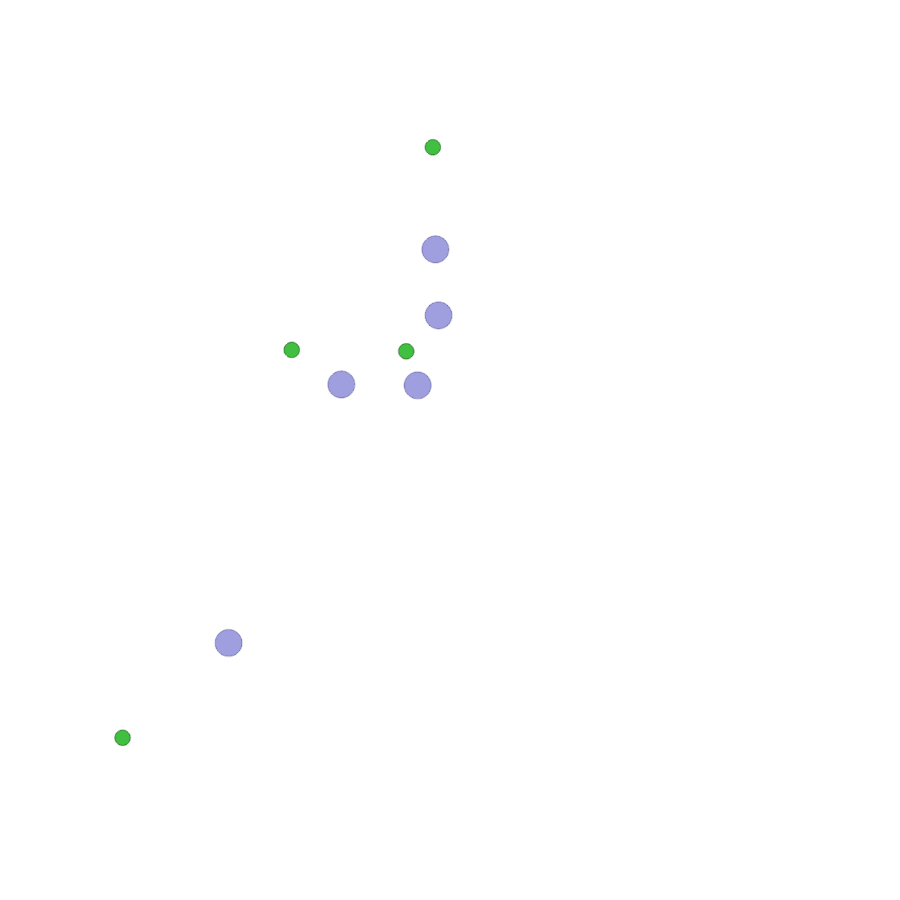
\includegraphics[width=\textwidth]{figs/dispersion.png}
        \caption{Dispersion}
        \label{fig:dispersion}
    \end{subfigure}
    \begin{subfigure}[b]{0.24\textwidth}
        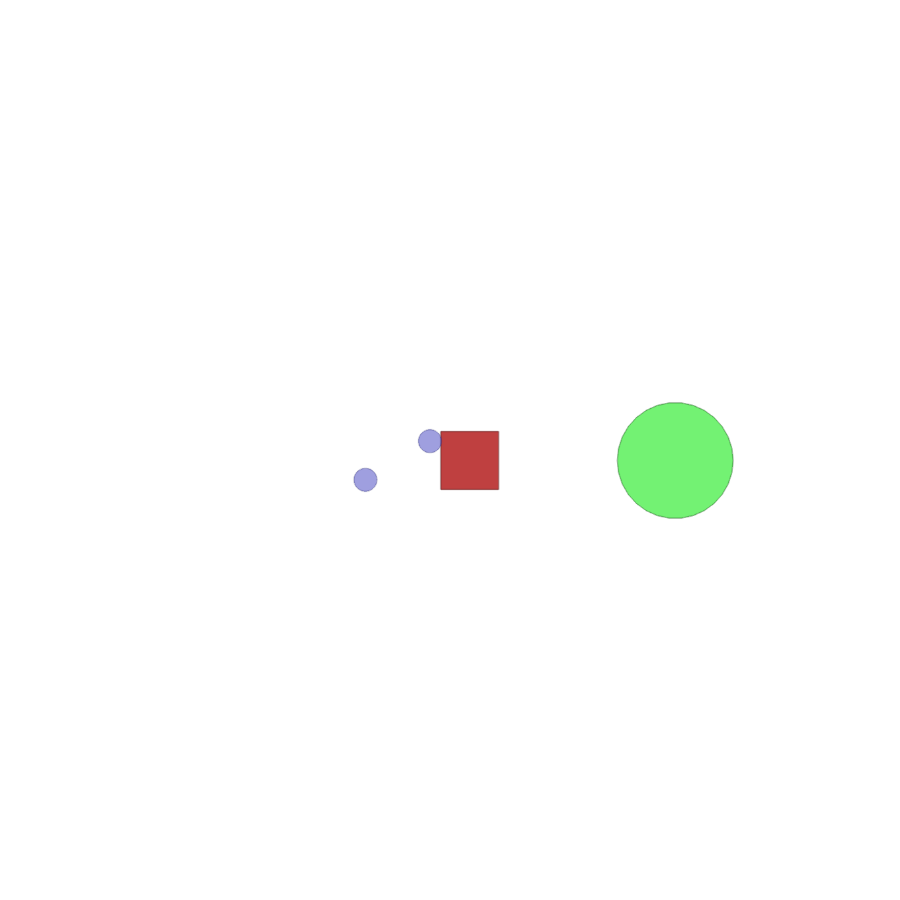
\includegraphics[width=\textwidth]{figs/transport.png}
        \caption{Transport}
        \label{fig:transport}
    \end{subfigure}
    \begin{subfigure}[b]{0.24\textwidth}
        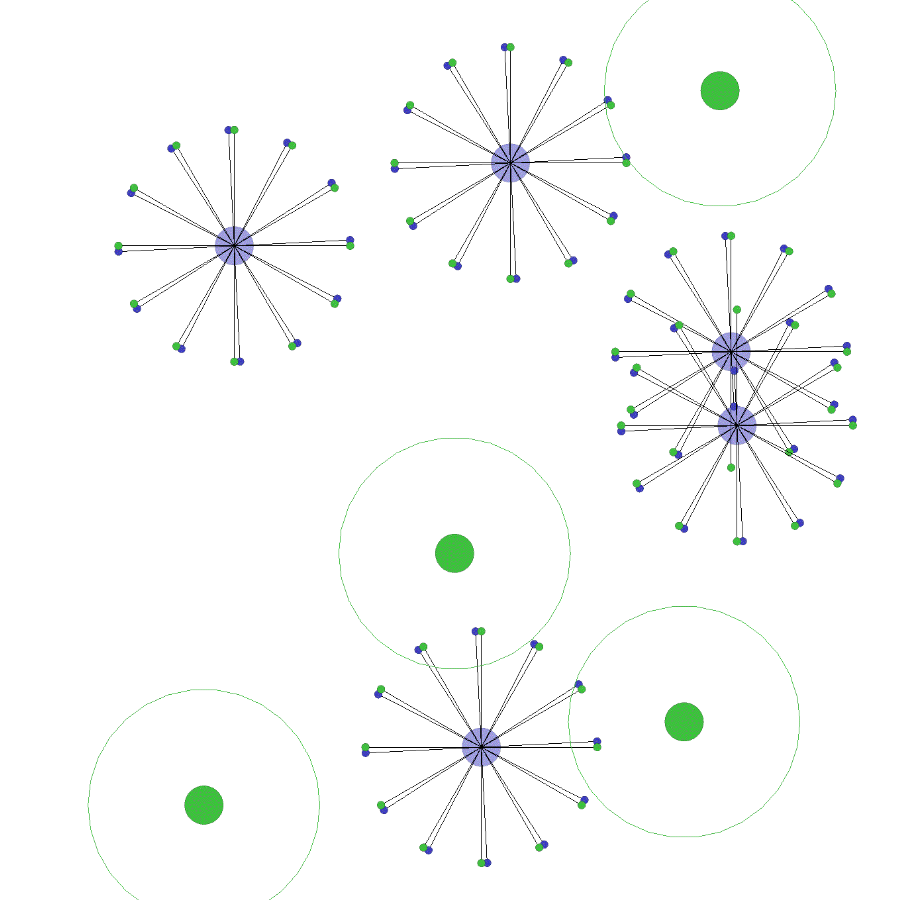
\includegraphics[width=\textwidth]{figs/discovery.png}
        \caption{Discovery}
        \label{fig:discovery}
    \end{subfigure}
    \begin{subfigure}[b]{0.24\textwidth}
        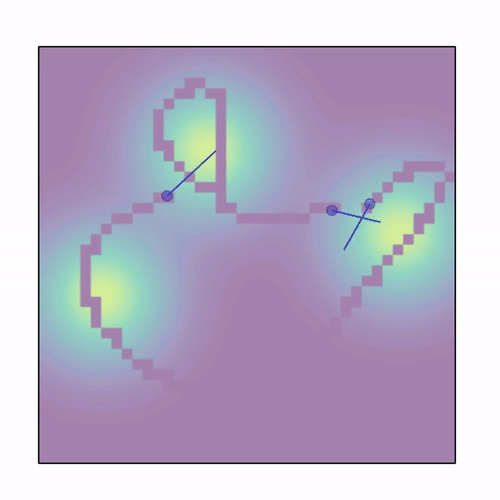
\includegraphics[width=\textwidth]{figs/sampling.png}
        \caption{Sampling}
        \label{fig:sampling}
    \end{subfigure}
    \caption{VMAS environments used in the experiments.}\label{fig:scenarios}
\end{figure}

\section{Environments}\label{apx:scenarios}

In this section, we provide a detailed discussion of the environment and scenarios used to test the \fname{} algorithm. Specifically, we utilize four vectorized environments available as part of VMAS.

VMAS is a differentiable simulator designed for various multi-agent tasks. These tasks are built on top of a differentiable physics engine, resulting in differentiable transition functions for all tasks. However, the reward function is non-differentiable. To address this limitation, we created custom reward functions, where possible, to replicate the non-differentiable ones provided by VMAS. Consequently, some scenarios are compatible with all tested algorithms (PPO, SHAC, and \fname{}), while others are only applicable to PPO and \fname{}.

Furthermore, the observations produced by VMAS are often only partial representations of the full state. While in some cases these observations are sufficient to predict the next observations, in others they are not. In such cases, \fname{} is expected to face challenges, as the world model is trained using only partial information. In contrast, SHAC computes gradients using access to the full world state. We chose to retain this limitation to better reflect the behavior of \fname{} in more realistic environments.

\subsection{Dispersion}
In the Dispersion task, $n$ agents must reach $n$ randomly placed goals. In \Cref{fig:dispersion}, the agents are represented by blue dots, while the goals are depicted as green dots.

Each agent has a continuous 2-dimensional action space, bounded between $-1$ and $1$, to represent acceleration along the x- and y-axes, respectively. Each agent observes its own position, velocity, and relative position to each goal. As a consequence, the world model has sufficient information to accurately predict the next states.

Each agent receives a reward of $1$ upon reaching a goal, making the maximum possible reward $n$. While the transition function is differentiable, the reward function is not. Consequently, only PPO and \fname{} are applicable to this scenario.

\subsection{Transport}
In the Transport problem, $n$ agents work together to push a package to a randomly placed target location. In \Cref{fig:transport}, the agents are represented by blue dots, the package is shown as a red square, and the goal is depicted as a green circle. The more agents collaborate to push the package, the faster they can reach the goal and achieve the maximum reward.

Each agent has a continuous 2-dimensional action space, bounded between $-1$ and $1$, to represent acceleration along the x- and y-axes, respectively. Each agent observes its own position, velocity, the relative position to the package, and the relative position between the package and the goal. As a consequence, the world model has sufficient information to accurately predict the next states.

Each agent receives a reward proportional to the distance between the initial position of the package and the goal. Consequently, the maximum reward corresponds to the distance between the package and the goal. Since the maximum reward varies across environments, we only plot a reference line representing good performance. Although this reward function is differentiable, the implementation provided by VMAS is not. Therefore, we created a custom reward function to replicate the original one used by all algorithms (\fname{}, SHAC, and PPO).


\subsection{Dicsovery}
In the Discovery task, $n$ agents aim to collect as many randomly placed goals as possible. When they successfully collect $k$ goals, another $k$ goals are randomly placed. To collect a goal, at least $s$ agents must be in proximity to it. In \Cref{fig:discovery}, the agents are represented by blue dots, while the goals are depicted as green dots. The proximity area is indicated by a dashed circle. In our experiments, we set $s=2$ and $k=7$ when $n > 1$. When $n = 1$, we set $s=1$ and $k=7$.

Each agent has a continuous 2-dimensional action space, bounded between $-1$ and $1$, to represent acceleration along the x- and y-axes, respectively. Each agent observes its own position, velocity, and lidar measurements of other agents and goals. As a consequence, the world model lacks sufficient information to accurately predict the next states. Specifically, the goal positions are not directly observed but are instead sensed through the lidar measurements. We believe this limitation significantly affects the performance of \fname{}.

Each agent receives a reward of $1$ when it collects a goal. Thus, the maximum reward depends on the amount of time the agents have to collect the goals. For early stopping purposes, we set the maximum reward to $k$. Additionally, the reference line is set to $k$. While the transition function is differentiable, the reward function is not. Therefore, only PPO and \fname{} are applicable to this scenario.

\subsection{Sampling}
In the Sampling task, $n$ agents must collect rewards from a grid. The rewards are sampled from $k$ Gaussian distributions. In \Cref{fig:sampling}, the agents are represented by blue dots, while the $k$ reward-generating Gaussians are displayed as a scalar field, where the intensity of the color represents the respective reward value.

Each agent has a continuous 2-dimensional action space, bounded between $-1$ and $1$, to represent acceleration along the x- and y-axes, respectively. Each agent observes its own position, velocity, lidar values from other agents, and rewards in a 3x3 grid around itself. As a consequence, the world model lacks sufficient information to accurately predict the next states. Specifically, it does not have access to the full reward distribution. We believe this limitation significantly affects the performance of \fname{}.

Each agent receives a reward equal to the value of the reward in the grid cell where it is located. Thus, the maximum reward depends on the placement of the Gaussians. Since the maximum reward varies across environments, we only plot a reference line representing good performance. While the reward function is differentiable, the one provided by VMAS is not. Therefore, we created a custom reward function to match the original one used by all algorithms (\fname{}, SHAC, and PPO).



